This section solves the middle layer to arrive at \figref{midlayer}.
\begin{figure}[h]
	\centering
	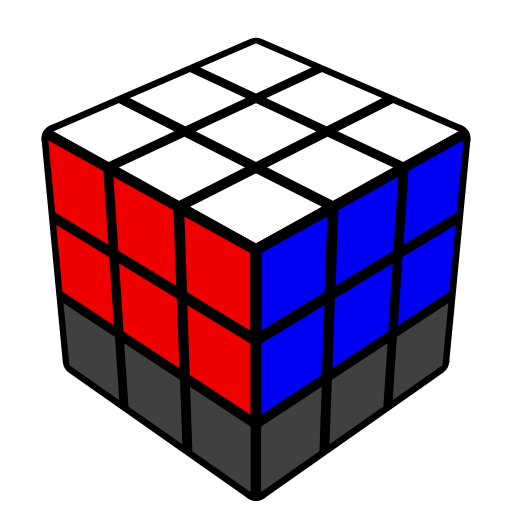
\includegraphics[width=0.3\textwidth]{midlayer.png}
	\caption{Solved middle layer}\label{fig:midlayer}
\end{figure}
\begin{enumerate}
	\item Flip the cube so that the white face is on the bottom. This allows you to observe the bottom (now top) layer easily.
	\item Find an edge on the new top layer that belongs in the middle layer.
	\item Align the side of that edge with the corresponding centre on the middle layer.
	\item The top face of the edge will be in one of the following configurations. Holding the edge in front of you, perform the appropriate algorithm:\begin{enumerate}
		\item Matches the left centre (as in \figref{midconf1}); do \alg{U'L'ULUFU'F'}.
		\item Matches the right centre (as in \figref{midconf2}); do \alg{URU'R'U'F'UF}.
	\end{enumerate}
\begin{figure}[h]
	\centering
	\begin{subfigure}[b]{0.3\textwidth}
		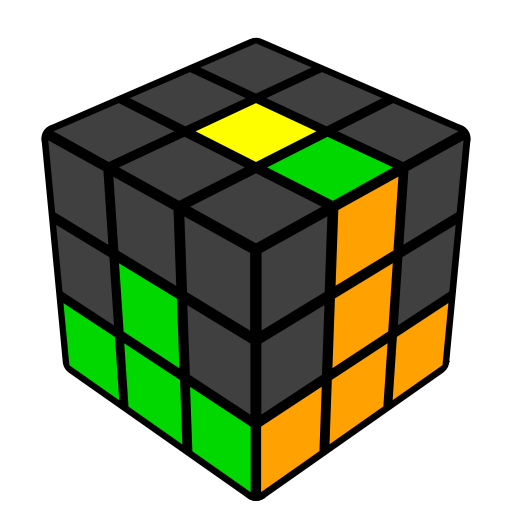
\includegraphics[width=\textwidth]{midconf1.png}
		\caption{Matches left}\label{fig:midconf1}
	\end{subfigure}
	\begin{subfigure}[b]{0.3\textwidth}
		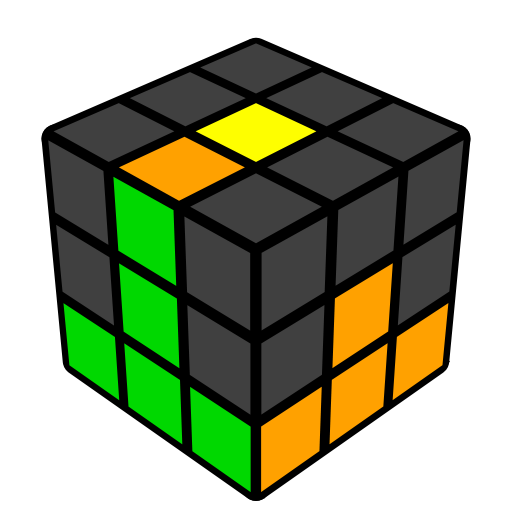
\includegraphics[width=\textwidth]{midconf2.png}
		\caption{Matches right}\label{fig:midconf2}
	\end{subfigure}
	\caption{Possible configurations of the middle edge.}
\end{figure}
	\item Repeat from step 1 until the middle layer is done.
	\item Flip the cube back to white on top.
\end{enumerate}
